\chapter{Results}

In this chapter will be presented the results of the experiments \nameExperimentI{} and \nameExperimentII{}, along side with a discussion of the impact on the lift and similarity distributions of these experiments relative to the OT without the clustering.

\section{Experiment \nameExperimentI}

As seen on \ref{ch:experiment-i} this experiment was the one that creates sub-runs of the OT for each cluster in the portfolio. Also, it had to be created some heuristics to deal with clusters that did not have enough data to run. Using the "manually clustering", as discussed on \ref{ch:cluster-algorithm} the summary of the lift gain (how much the lift on the first decile increased or decreased relative to the OT without clustering) is presented on Table \ref{table:lift_gain_exp-i}. 

The cells are colored to better understand the gains. The green ones represent a positive gain, the light red ones represent a sightly negative gain, the dark red ones represent a considerable negative gain, the white represent that the lift did not change, and finally the orange ones are the outliers which were defined using the interquartile range rule \cite{upton1996understanding}. 

There are, also, some studies that are bolded. They represent the studies that brought up the hypothesis of this work, as discussed on the Introduction, they had two or more high density areas on the similarity distribution plot, meaning that, they can have more than one profile on their portfolio.

\begin{table}[h]
\centering
\begin{tabular}{|c|c|c|c|}
\hline
\textbf{Study} & \textbf{Lift Gain (\%)}        & \textbf{Study} & \textbf{Lift Gain (\%)}        \\ \hline
1              & \cellcolor[HTML]{ff514d}-12,09 & 15             & \cellcolor[HTML]{ff514d}-13,26 \\ \hline
2              & \cellcolor[HTML]{8ed08e}16,67  & \textbf{16}    & \cellcolor[HTML]{ff514d}-20,00 \\ \hline
3              & \cellcolor[HTML]{8ed08e}0,89   & \textbf{17}    & \cellcolor[HTML]{ffccc9}-4,28  \\ \hline
4              & 0,00                           & 18             & \cellcolor[HTML]{ff514d}-13,06 \\ \hline
5              & \cellcolor[HTML]{ffccc9}-0,14  & 19             & \cellcolor[HTML]{ff514d}-15,42 \\ \hline
6              & \cellcolor[HTML]{ff514d}-17,28 & 20             & \cellcolor[HTML]{8ed08e}0,57   \\ \hline
7              & \cellcolor[HTML]{ff514d}-12,44 & 21             & \cellcolor[HTML]{ff514d}-33,95 \\ \hline
\textbf{8}     & \cellcolor[HTML]{ffccc9}-5,17  & 22             & 0,00                           \\ \hline
\textbf{9}     & \cellcolor[HTML]{ff514d}-27,78 & 23             & \cellcolor[HTML]{ff514d}-28,16 \\ \hline
\textbf{10}    & \cellcolor[HTML]{8ed08e}6,25   & 24             & \cellcolor[HTML]{ffce93}200,01 \\ \hline
11             & \cellcolor[HTML]{ff514d}-17,75 & \textbf{25}    & \cellcolor[HTML]{ff514d}-12,77 \\ \hline
12             & \cellcolor[HTML]{ffccc9}-1,01  & 26             & \cellcolor[HTML]{ff514d}-29,35 \\ \hline
13             & \cellcolor[HTML]{ff514d}-6,93  & 27             & \cellcolor[HTML]{ffccc9}-0,08  \\ \hline
14             & \cellcolor[HTML]{ffccc9}-1,16  &                &                                \\ \hline
\end{tabular}
\caption{Summary of the first-decile lift gains for Experiment \nameExperimentI}
\label{table:lift_gain_exp-i}
\end{table}

We can see that only 5 studies had positive impact on the lift, and one of them is an outlier. The majority of the studies had a negative impact - 6 of them were sightly negative and 14 worsened the lift considerably. It is important to notice that two studies did not present any changes on the lift with the clustering.

The Figure \ref{fig:lift-hist-plot-exp-i} shows a histogram of the lift gain for the studies excluding the outliers. We can see that the mean lift gain for \nameExperimentI{} is \textbf{-9.871 \%}.

\begin{figure}[h]
   \centering
   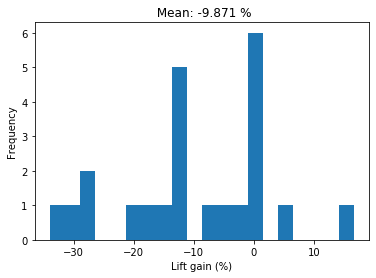
\includegraphics[width=\linewidth]{fig/ch4-lift-hist-plot-exp-i.png}
   \caption{Histogram plot of the studies' lift gain for experiment \nameExperimentI{}. Source: Author}
   \label{fig:lift-hist-plot-exp-i}
\end{figure}

\section{Experiment \nameExperimentII{}}

Now for the second experiment, which was the simple use of the clustering information as another feature. Using the same color scheme as Table \ref{table:lift_gain_exp-i}, Table \label{table:lift_gain_exp-ii} shows the summary of the lift gains for the experiment \nameExperimentII{}.

\begin{table}[h]
\centering
\begin{tabular}{|c|c|c|c|}
\hline
\textbf{Study} & \textbf{Lift Gain (\%)}        & \textbf{Study} & \textbf{Lift Gain (\%)}        \\ \hline
1              & \cellcolor[HTML]{8ed08e}4,40   & 15             & \cellcolor[HTML]{8ed08e}0,46   \\ \hline
2              & \cellcolor[HTML]{ff514d}-8,33  & \textbf{16}    & \cellcolor[HTML]{ff514d}-6,58  \\ \hline
3              & \cellcolor[HTML]{ffce93}23,65  & \textbf{17}    & \cellcolor[HTML]{ffce93}-46,08 \\ \hline
4              & 0,00                           & 18             & \cellcolor[HTML]{ffccc9}-1,87  \\ \hline
5              & \cellcolor[HTML]{8ed08e}1,49   & 19             & \cellcolor[HTML]{8ed08e}3,58   \\ \hline
6              & \cellcolor[HTML]{ffce93}-28,33 & 20             & \cellcolor[HTML]{ff514d}-11,28 \\ \hline
7              & \cellcolor[HTML]{8ed08e}12,50  & 21             & \cellcolor[HTML]{ffccc9}-2,64  \\ \hline
\textbf{8}     & \cellcolor[HTML]{8ed08e}16,84  & 22             & \cellcolor[HTML]{8ed08e}1,23   \\ \hline
\textbf{9}     & \cellcolor[HTML]{8ed08e}12,80  & 23             & \cellcolor[HTML]{ffccc9}-0,14  \\ \hline
\textbf{10}    & \cellcolor[HTML]{8ed08e}18,59  & 24             & \cellcolor[HTML]{ffce93}300,02 \\ \hline
11             & \cellcolor[HTML]{ff514d}-7,84  & \textbf{25}    & \cellcolor[HTML]{8ed08e}4,90   \\ \hline
12             & \cellcolor[HTML]{ffccc9}-0,15  & 26             & \cellcolor[HTML]{ffccc9}-0,77  \\ \hline
13             & \cellcolor[HTML]{8ed08e}0,68   & 27             & \cellcolor[HTML]{8ed08e}1,21   \\ \hline
14             & \cellcolor[HTML]{8ed08e}7,30   &                &                                \\ \hline
\end{tabular}
\caption{Summary of the first-decile lift gains for Experiment \nameExperimentII}
\label{table:lift_gain_exp-ii}
\end{table}

We can see that, differently from \nameExperimentI{}, the majority of the studies had positive gain (16 studies, to be exactly), two of them are outliers. Only 4 studies were considerably worse on the lift gain and 5 sightly worse, a total of 9 studies. Only one study did not presented any change on the lift and, this time, 4 were outliers (2 positives and 2 negatives).

The Figure \ref{fig:lift-hist-plot-exp-ii} shows a histogram of the lift gain for the studies excluding the outliers. We see that the mean lift gain for \nameExperimentII{} is \textbf{2.016 \%}.

\begin{figure}[h]
   \centering
   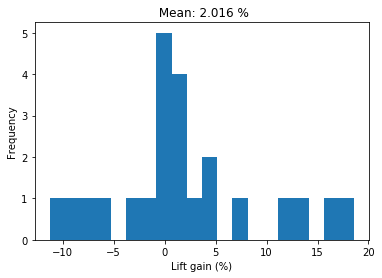
\includegraphics[width=\linewidth]{fig/ch4-lift-hist-plot-exp-ii.png}
   \caption{Histogram plot of the studies' lift gain for experiment \nameExperimentII{}. Source: Author}
   \label{fig:lift-hist-plot-exp-ii}
\end{figure}

\section{Similarity distributions}

Now let us look at some of the similarity distributions plots for both experiments. These plots will have three curves:
% TODO check the colors of this dist plots i think the port and market is switched
the market similarity in green, the holdout set in orange, and the portfolio in blue. Each topic of this section will address a group represented by the colors in the lift gain summary tables. 

\subsection{No change on the lift}

In both experiments there were studies that do not had any variation on the lift. \underline{Study 4} appeared on both. Figure \ref{fig:study-4-comparsion} shows the similarity distribution plots for Study 6. The first row is the run of the OT without the clustering, and the second row is with the clustering. On the left is presented the \nameExperimentI{} experiment and on the right \nameExperimentII{}. There is, also, on the information about the size of the sets in the study. This is a study with around 4600 companies on the portfolio (1100 are the Holdout set) and a market around 220 thousand companies, meaning that the portfolio correspond to approximately 1.5\% of the companies on the study.
% TODO Can I show the port size, holdout size and market size?

\begin{figure}[h]
   \centering
   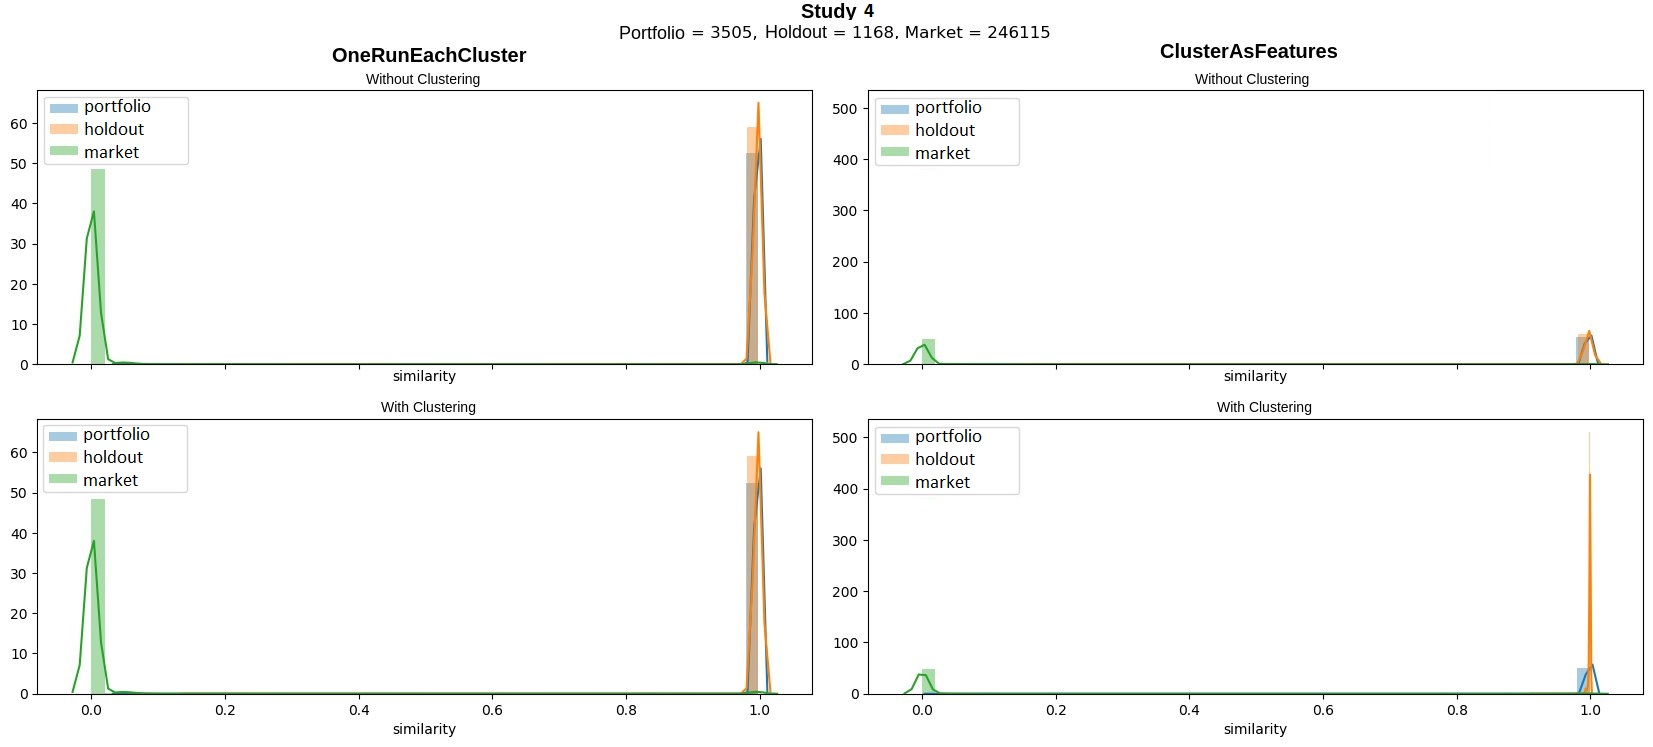
\includegraphics[width=\linewidth]{fig/ch4-study-4-comparsion.jpg}
   \caption{Similarity distribution plot for Study 4 for both experiments. Source: Author}
   \label{fig:study-4-comparsion}
\end{figure}

\begin{figure}[h]
   \centering
   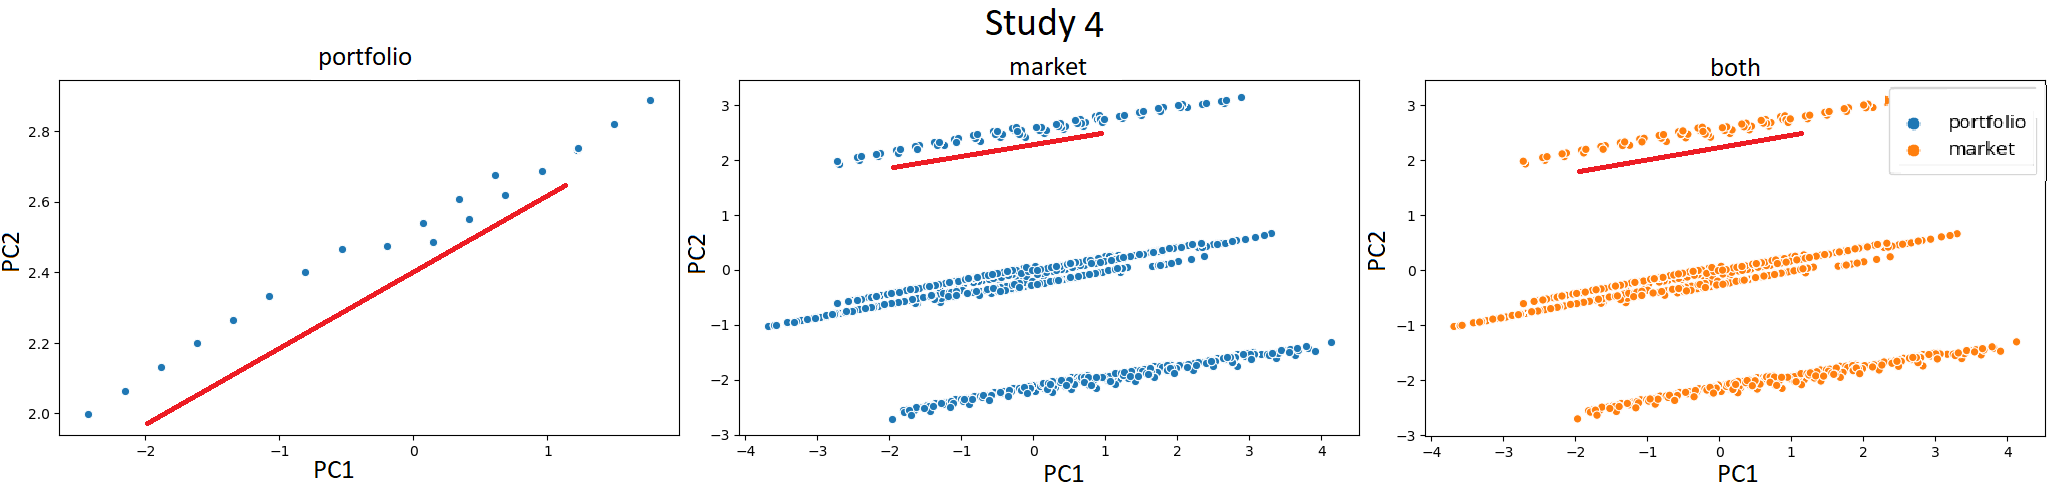
\includegraphics[width=\linewidth]{fig/ch4-study-4-pca-plot.png}
   \caption{PCA plot for Study 4. The red line is the same on the three plots. Source: Author}
   \label{fig:study-4-pca-plot}
\end{figure}

We can see that on \nameExperimentI{} the similarity distributions with and without clustering are virtually the same. This is better understood when you look at the number of clusters in its portfolio. Figure \ref{fig:study-4-pca-plot} shows its PCA plot. There is only a single cluster on the portfolio, consequentially, the result of this cluster is the same of the aggregated output and, at the same time, the result without clustering.

On \nameExperimentII{}, however, there is a difference on the distributions between the with and without the clustering. Basically, the holdout set changed its distribution. In this experiment the OT scored this companies with really close scores, in other words, their standard deviation decreased. But, even though the scores of the companies (and possibly the ordering) of the holdout set changed, the lift kept the same because of the way to calculate this metric. The same number of companies (of the holdout set) on the first decile occurred in the run without the clustering and in with the clustering, thus the value of the lift is the same for both runs.

Another study that had a zero lift gain was \underline{Study 22}, in the \nameExperimentI{} experiment. Figure \ref{fig:study-22-clusters-simi-plot} shows the similarity distribution plots for the clusters' runs of this study.

\begin{figure}[h]
   \centering
   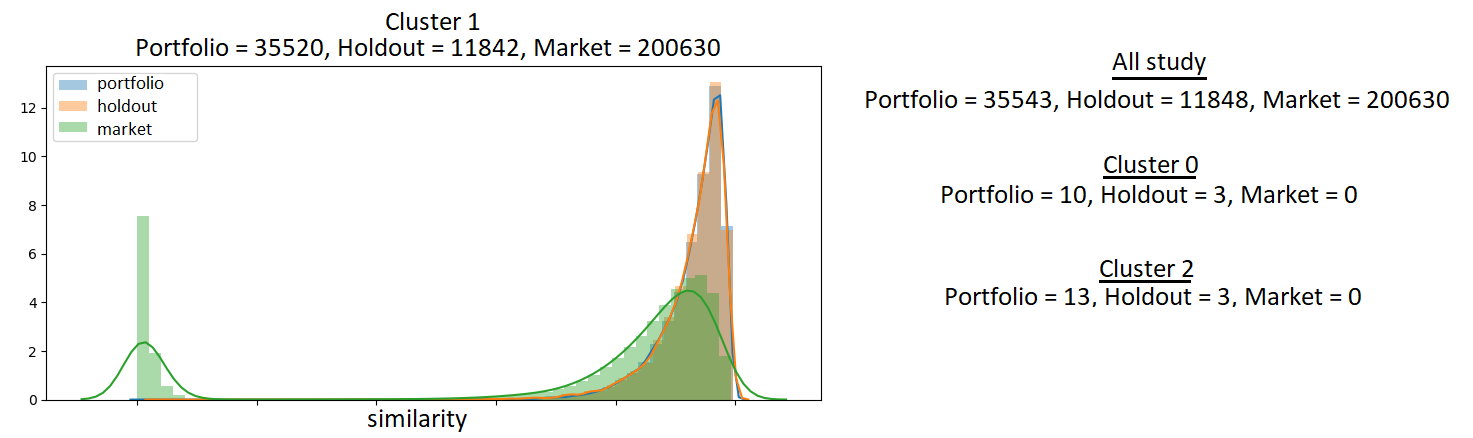
\includegraphics[width=\linewidth]{fig/ch4-study-22-clusters-simi-plot.png}
   \caption{Similarity distribution plot for the clusters' runs of Study 22 on experiment \nameExperimentI{}. Source: Author}
   \label{fig:study-22-clusters-simi-plot}
\end{figure}

Although this study has 3 clusters on the portfolio, only Cluster 1 has the minimum data to a valid run. Cluster 0 and Cluster 2 do not have companies on the Market, so the 16 companies of the former and 13 companies of latter are discarded. Since they represent less than 0.001 \% of the overall data of the study, the behavior is practically the same as Study 4, thus, for the same reason, the lift is the same for both runs (with and without clustering).

\subsection{marginal increase and decrease on the lift}

we see that on figure ... and figure .... for both experiments the simi distribuion was almost the same as without clustering

\subsection{considerable  increase and decrease on the lift}

we can see the holdout set skew to left and right on increase and deacrease.... figure .. shows it

\subsection{outliers}

study ... had an huge improve on the lift , and it appear in both experiments. figure show its simi dist. 



\subsection{studies that had multiple profiles}

no obvious pattern, actually no pattern at all

\section{Experiment \nameExperimentII{} with other clustering algorithms}

Seing the performance of the bad performance of experiment I it was decided to not continue the work with it, then it was decided to test exp 2 with the other clusrint algoriths showd in figure ...

figure ... shows the histogram of the lift gains for the three algorithsm






